\documentclass[11pt]{article}
% Shared preamble for the pyMack LST documentation set.
% Used by: mean_boundary_layer.tex, disturbance_equations.tex,
%          numerical_methods.tex, validation.tex
% Each document begins with:  \documentclass[11pt]{article}% Shared preamble for the pyMack LST documentation set.
% Used by: mean_boundary_layer.tex, disturbance_equations.tex,
%          numerical_methods.tex, validation.tex
% Each document begins with:  \documentclass[11pt]{article}% Shared preamble for the pyMack LST documentation set.
% Used by: mean_boundary_layer.tex, disturbance_equations.tex,
%          numerical_methods.tex, validation.tex
% Each document begins with:  \documentclass[11pt]{article}\input{lst_preamble}
\usepackage[margin=1in]{geometry}
\usepackage{amsmath,amssymb,mathtools}
\usepackage{booktabs}
\usepackage{enumitem}
\usepackage{array}
\usepackage{graphicx}
\usepackage{caption}
\usepackage{xcolor}
\usepackage[hidelinks]{hyperref}

\graphicspath{{figures/}}
\captionsetup{font=small,labelfont=bf}

\definecolor{kicol}{RGB}{31,143,107}
\definecolor{boxbg}{RGB}{238,246,242}
\definecolor{rmkbg}{RGB}{244,244,244}

\newcommand{\plain}[1]{\par\smallskip\noindent{\color{kicol}\textbf{In plain words.}}\ \textit{#1}\par\smallskip}
\newcommand{\problembox}[1]{%
  \par\smallskip\noindent\fcolorbox{kicol}{boxbg}{%
  \parbox{0.965\linewidth}{\smallskip\textbf{\color{kicol}What problem is solved here.}\ \ #1\smallskip}}\par\smallskip}
\newcommand{\remark}[2]{%
  \par\smallskip\noindent\colorbox{rmkbg}{%
  \parbox{0.965\linewidth}{\smallskip\footnotesize\textbf{#1}\ \ #2\smallskip}}\par\smallskip}
\newcommand{\bridge}[1]{\par\noindent\textit{#1}\par\medskip}

\newcommand{\D}{\mathrm{D}}
\newcommand{\imag}{\mathrm{i}}
\newcommand{\Real}{\operatorname{Re}}
\newcommand{\Imag}{\operatorname{Im}}
\newcommand{\Mae}{M_e}
\newcommand{\Ree}{\mathit{Re}}
\renewcommand{\bar}[1]{\overline{#1}}
\newcommand{\hatu}{\hat{u}}
\newcommand{\hatv}{\hat{v}}
\newcommand{\hatT}{\hat{T}}
\newcommand{\hatp}{\hat{p}}
\newcommand{\hatq}{\hat{q}}
\newcommand{\nuR}{\nu_{\!R}}

\usepackage[margin=1in]{geometry}
\usepackage{amsmath,amssymb,mathtools}
\usepackage{booktabs}
\usepackage{enumitem}
\usepackage{array}
\usepackage{graphicx}
\usepackage{caption}
\usepackage{xcolor}
\usepackage[hidelinks]{hyperref}

\graphicspath{{figures/}}
\captionsetup{font=small,labelfont=bf}

\definecolor{kicol}{RGB}{31,143,107}
\definecolor{boxbg}{RGB}{238,246,242}
\definecolor{rmkbg}{RGB}{244,244,244}

\newcommand{\plain}[1]{\par\smallskip\noindent{\color{kicol}\textbf{In plain words.}}\ \textit{#1}\par\smallskip}
\newcommand{\problembox}[1]{%
  \par\smallskip\noindent\fcolorbox{kicol}{boxbg}{%
  \parbox{0.965\linewidth}{\smallskip\textbf{\color{kicol}What problem is solved here.}\ \ #1\smallskip}}\par\smallskip}
\newcommand{\remark}[2]{%
  \par\smallskip\noindent\colorbox{rmkbg}{%
  \parbox{0.965\linewidth}{\smallskip\footnotesize\textbf{#1}\ \ #2\smallskip}}\par\smallskip}
\newcommand{\bridge}[1]{\par\noindent\textit{#1}\par\medskip}

\newcommand{\D}{\mathrm{D}}
\newcommand{\imag}{\mathrm{i}}
\newcommand{\Real}{\operatorname{Re}}
\newcommand{\Imag}{\operatorname{Im}}
\newcommand{\Mae}{M_e}
\newcommand{\Ree}{\mathit{Re}}
\renewcommand{\bar}[1]{\overline{#1}}
\newcommand{\hatu}{\hat{u}}
\newcommand{\hatv}{\hat{v}}
\newcommand{\hatT}{\hat{T}}
\newcommand{\hatp}{\hat{p}}
\newcommand{\hatq}{\hat{q}}
\newcommand{\nuR}{\nu_{\!R}}

\usepackage[margin=1in]{geometry}
\usepackage{amsmath,amssymb,mathtools}
\usepackage{booktabs}
\usepackage{enumitem}
\usepackage{array}
\usepackage{graphicx}
\usepackage{caption}
\usepackage{xcolor}
\usepackage[hidelinks]{hyperref}

\graphicspath{{figures/}}
\captionsetup{font=small,labelfont=bf}

\definecolor{kicol}{RGB}{31,143,107}
\definecolor{boxbg}{RGB}{238,246,242}
\definecolor{rmkbg}{RGB}{244,244,244}

\newcommand{\plain}[1]{\par\smallskip\noindent{\color{kicol}\textbf{In plain words.}}\ \textit{#1}\par\smallskip}
\newcommand{\problembox}[1]{%
  \par\smallskip\noindent\fcolorbox{kicol}{boxbg}{%
  \parbox{0.965\linewidth}{\smallskip\textbf{\color{kicol}What problem is solved here.}\ \ #1\smallskip}}\par\smallskip}
\newcommand{\remark}[2]{%
  \par\smallskip\noindent\colorbox{rmkbg}{%
  \parbox{0.965\linewidth}{\smallskip\footnotesize\textbf{#1}\ \ #2\smallskip}}\par\smallskip}
\newcommand{\bridge}[1]{\par\noindent\textit{#1}\par\medskip}

\newcommand{\D}{\mathrm{D}}
\newcommand{\imag}{\mathrm{i}}
\newcommand{\Real}{\operatorname{Re}}
\newcommand{\Imag}{\operatorname{Im}}
\newcommand{\Mae}{M_e}
\newcommand{\Ree}{\mathit{Re}}
\renewcommand{\bar}[1]{\overline{#1}}
\newcommand{\hatu}{\hat{u}}
\newcommand{\hatv}{\hat{v}}
\newcommand{\hatT}{\hat{T}}
\newcommand{\hatp}{\hat{p}}
\newcommand{\hatq}{\hat{q}}
\newcommand{\nuR}{\nu_{\!R}}


\title{\textbf{Numerical Methods: Eigenvalue Assembly and the Shooting Solver}\\[3pt]
\large Two routes to the compressible boundary-layer stability eigenvalue: the global\\
spectral (Chebyshev collocation) assembly and the local shooting solver of \texttt{pyMack}}
\author{\texttt{pyMack} technical documentation}
\date{\today}

\begin{document}
\maketitle
\tableofcontents
\bigskip

%=====================================================================
\section{Scope: the problem to be solved and the two routes}\label{sec:scope}
%=====================================================================
The companion document \emph{Derivation of the Disturbance Equations} closes with three objects: the
four linearised disturbance ODEs for $\hatq(y)=(\hatu,\hatv,\hatT,\hatp)$, their operator form
$\mathsf L(\alpha;y,\D)\,\hatq=c\,\mathsf M(\alpha;y)\,\hatq$, and the statement that, upon replacing
the continuous derivative by the discretised derivative operator ($\D\to D_1$, $\D^2\to D_2$), this
pencil becomes the finite generalised eigenvalue problem $A(\alpha)\boldsymbol\phi=c\,B(\alpha)\,
\boldsymbol\phi$. The present document supplies every constructive detail behind that statement: the
grid, the differentiation matrices, the block-by-block assembly, the boundary-condition rows, the
eigenvalue algorithms, and the identification of the physical mode. It also documents a second,
independent numerical route to the same eigenvalue.

\paragraph{What is sought.} For fixed flow parameters $(\Mae,\Ree)$ the disturbance equations admit
non-trivial solutions only at isolated eigenvalues, and these eigenvalues are the entire objective of
the computation:
\begin{itemize}[nosep,leftmargin=1.6em]
  \item \emph{Temporal problem}: given a real wavenumber $\alpha$, find the complex phase speed $c$
        and mode shape; the temporal growth rate is $\omega_i=\alpha c_i$.
  \item \emph{Spatial problem}: given a real frequency $\omega$, find the complex wavenumber
        $\alpha$ and mode shape; the spatial growth rate is $\sigma=-\alpha_i$.
\end{itemize}
Every quantity the framework ultimately delivers is assembled from repeated eigenvalue solves: the
\emph{neutral curve} is the zero-growth locus $c_i(R,\alpha)=0$ traced over a parameter sweep; the
\emph{$N$-factor} is the streamwise integral of the spatial growth rate at fixed physical frequency;
and the transition estimate is the empirical correlation $N\approx9$--$11$
\cite{smith1956,vaningen1956}. The numerical task is therefore to evaluate eigenpairs reliably,
including the rejection of spurious eigenvalues, and cheaply enough to sweep them by the thousands.

\paragraph{Two routes.} Numerical methods for this problem divide into two classical families
\cite{malik1990}: \emph{boundary-value methods}, which discretise the ODEs globally and obtain all
eigenvalues of the resulting matrix pencil at once without prior knowledge of the spectrum, and
\emph{initial-value (shooting) methods}, which integrate the ODEs across the layer and locate one
eigenvalue by enforcing the boundary conditions, requiring a good initial guess but very little
memory. \texttt{pyMack} implements one of each: \textbf{Part~A} is the spectral boundary-value route
(Chebyshev collocation, block assembly, and dense eigensolves), used for spectrum surveys,
neutral curves, and $N$-factors; \textbf{Part~B} is the shooting route
(\texttt{pymack/temporal\_shooting.py}), the classical procedure of Mack \cite{mack1984} in the
formulation of \"Ozgen \& K{\i}rcal{\i} \cite{ozgen2008}, used to refine and independently verify a
mode found by Part~A. Both return the same physical eigenvalue; their agreement is a strong check that
a computed mode is physics rather than discretisation artifact. Every equation, coefficient, and
default below is transcribed from the code, cited by file.

\paragraph{Notation.} Overbars denote mean (base-flow) quantities; hats denote complex disturbance
amplitudes. The continuous amplitude is $\hatq(y)=(\hatu,\hatv,\hatT,\hatp)$; its discrete (stacked,
grid-sampled) form is $\boldsymbol\phi$. A prime on a mean quantity denotes
$\D\equiv\mathrm d/\mathrm dy$. The collocation order is $N$; the grid has $n=N{+}1$ points, so the
assembled matrices are $4n\times4n$, the size written $4(n{+}1)\times4(n{+}1)$ in the companion
document's indexing.
\begin{center}\footnotesize
\renewcommand{\arraystretch}{1.18}
\begin{tabular}{@{}ll@{\hspace{1.4em}}ll@{}}
\toprule
\multicolumn{2}{@{}l}{\textbf{Base flow \& transport}} & \multicolumn{2}{l}{\textbf{Disturbance / eigenvalue}}\\
$\bar U,\bar T,\bar\rho{=}1/\bar T$ & mean velocity, temp., density & $\hatq;\ \boldsymbol\phi$ & amplitude (continuous; discrete)\\
$\bar\mu,\bar\kappa$ & viscosity, conductivity & $\hatu,\hatv,\hatT,\hatp$ & velocity/temp./pressure amplitudes\\
$\Mae,\ \Ree,\ \mathit{Pr},\ \gamma$ & Mach, Reynolds, Prandtl, $c_p/c_v$ & $\alpha,\ \omega$ & wavenumber, frequency\\
$L^*,\ R{=}\sqrt{Re_x}$ & Mack length, Mack Reynolds number & $c{=}\omega/\alpha$ & complex phase speed; $c_r,c_i$ its parts\\
$\nuR{=}1/(\Ree\bar\rho)$ & viscous prefactor & $\omega_i{=}\alpha c_i;\ \sigma{=}-\alpha_i$ & temporal; spatial growth rate\\
$C{=}\bar\mu/\bar T$ & Chapman--Rubesin group & $N;\ n{=}N{+}1$ & collocation order; grid size\\
\bottomrule
\end{tabular}
\end{center}
\noindent{\footnotesize\textbf{Operator shorthands:}\ $D_1,D_2$ differentiation matrices;\
$\mathcal C_\kappa,\mathcal C_d,d_R$ conduction/dissipation prefactors;\ $\mathcal L_c$ conduction
operator;\ $A,B$ (temporal) and $C_0,C_1,C_2$ (spatial) operator blocks;\ $Y,\ M(c),\
\sigma_{\min}(c)$ (Part~B) shooting state, wall matrix, and its smallest singular value.\par}

%=====================================================================
\part*{Part A: The spectral (Chebyshev collocation) method}
\addcontentsline{toc}{section}{Part A: The spectral (Chebyshev collocation) method}
%=====================================================================
The disturbance equations are four coupled ODEs in $y$ with known base-flow coefficients but no
closed-form solution. Part~A converts them into a finite matrix pencil, solves the pencil for its
complete spectrum, identifies the physical mode, and sweeps the solve into neutral curves and
$N$-factors; this is the boundary-value route of Section~\ref{sec:scope}.

\section{Chebyshev collocation}\label{sec:cheb}
The first task is to replace the wall-normal derivative $\D$ by a finite matrix, so that the
disturbance ODEs become linear algebra and each continuous amplitude $\hatq(y)$ becomes the vector of
its values at chosen grid points.

\paragraph{Nodes and spectral accuracy.} For smooth functions a polynomial interpolant through
Chebyshev points converges exponentially with the polynomial degree
\cite{orszag1971,trefethen2000}, so few points yield many digits; this property makes spectral
collocation the natural discretisation for boundary-layer eigenvalue problems. The
Chebyshev--Gauss--Lobatto nodes on $[-1,1]$ are
\begin{equation}\label{eq:gll}
  \xi_j=\cos\!\Big(\frac{\pi j}{N}\Big),\quad j=0,1,\dots,N,
\end{equation}
clustering near the ends $\xi=\pm1$. The node ordering matters throughout what follows: $\xi_0=+1$
and $\xi_N=-1$, so the index runs from $+1$ down to $-1$.

\paragraph{The differentiation matrix.} Exactly one polynomial of degree $\le N$ passes through the
values $\{f(\xi_j)\}$; differentiating it and evaluating at the nodes is a linear operation,
$f'(\xi_j)\approx\sum_kD_{jk}f(\xi_k)$, with entries \cite{dons1995,trefethen2000}
(\texttt{spectral.py:chebyshev\_D})
\begin{equation}\label{eq:Dformula}
  D_{jk}=\frac{c_j}{c_k}\frac{(-1)^{j+k}}{\xi_j-\xi_k}\ (j\neq k),\qquad
  D_{jj}=-\!\!\sum_{k\neq j}D_{jk},\qquad c_0=c_N=2,\ c_{\text{else}}=1 .
\end{equation}
The diagonal is set so that each row sums to zero (a constant function has zero derivative), and
$c_0=c_N=2$ accounts for the doubled weight of the two endpoints. The matrix is dense because every
node's derivative uses every node's value; this is why the assembled stability matrices are dense. The
second derivative on $[-1,1]$ is the matrix square, $D_\xi^2=D_\xi D_\xi$, formed \emph{before} the
domain mapping below.

\paragraph{Mapping to the physical layer.} The flow occupies $y\in[0,y_{\max}]$ with resolution needed
at the \emph{wall}. The algebraic map of Malik \cite{malik1990} (\texttt{spectral.py:map\_domain}) is
\begin{equation}\label{eq:map}
  y(\xi)=L\,\frac{1+\xi}{1-\xi+2L/y_{\max}},\qquad L=\frac{y_{\max}}{6}\ \ (\text{stretching parameter}),
\end{equation}
which sends $\xi=+1$ (node $j{=}0$) to $y=y_{\max}$ (freestream) and $\xi=-1$ (node $j{=}N$) to $y=0$
(wall), placing roughly half the nodes below $y\approx L$ (Figure~\ref{fig:grid}). By the chain rule,
with $\xi_y=1/y_\xi$ and $\xi_{yy}=-y_{\xi\xi}/y_\xi^3$, the physical differentiation matrices are
\begin{equation}\label{eq:Dmats}
  D_1=\operatorname{diag}(\xi_y)\,D_\xi,\qquad
  D_2=\operatorname{diag}(\xi_y^2)\,D_\xi^2+\operatorname{diag}(\xi_{yy})\,D_\xi .
\end{equation}
Note that the chain rule acts on the computational second-derivative matrix $D_\xi^2$; the physical
$D_2$ is \emph{not} $D_1D_1$.

\paragraph{Domain height and resolution.} The truncation height must clear the boundary layer by a
wide margin and is therefore set as a multiple of the boundary-layer scale,
$y_{\max}=m\,(\delta^*/L^*)$, with $m\approx8$--$12$ for the wall-trapped second mode and larger
($m\approx35$--$45$) for the more diffuse first mode; the bare values $y_{\max}=6$/$12$ are only a
fallback. The default resolution is $N=128$ ($n=129$). Because the method is spectral, the eigenvalue
converges exponentially in $N$ \cite{orszag1971,trefethen2000}; at the default resolution the
worked-example eigenvalue of Section~\ref{sec:worked} is already converged to many digits.

\begin{figure}[H]\centering
  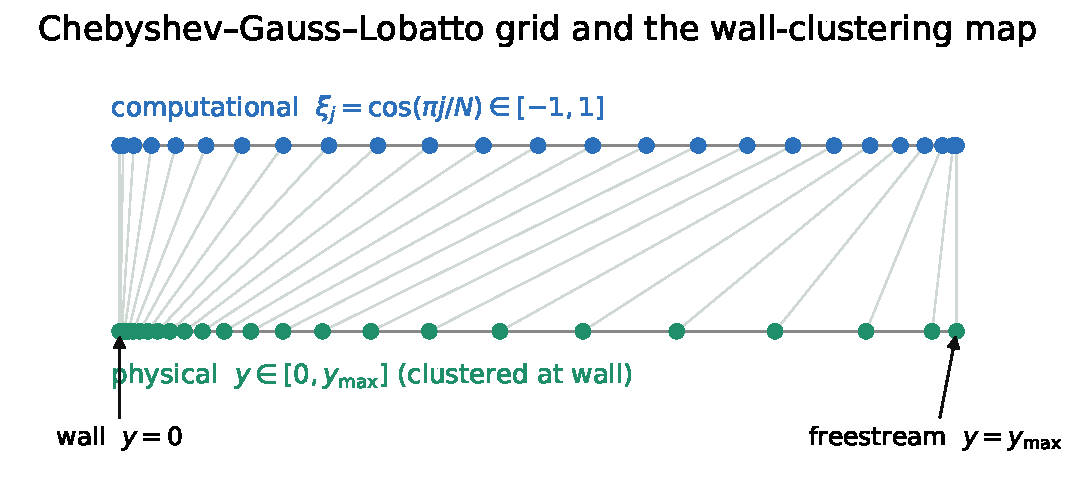
\includegraphics[width=0.92\linewidth]{fig_cheb_grid.pdf}
  \caption{The Chebyshev--Gauss--Lobatto nodes $\xi_j=\cos(\pi j/N)$ on $[-1,1]$ (top) map by
  Eq.~\eqref{eq:map} to the physical grid $y\in[0,y_{\max}]$ (bottom), clustering at the wall
  ($\xi=-1$) where the eigenfunctions vary fastest.}\label{fig:grid}
\end{figure}

\section{Assembling the operator and its boundary conditions}\label{sec:assemble}
The companion document closes with the operator pencil
\begin{equation}\label{eq:pencilA}
  \mathsf L(\alpha;y,\D)\,\hatq=c\,\mathsf M(\alpha;y)\,\hatq,\qquad
  \mathsf L=\mathsf A_2(y)\,\D^2+\mathsf A_1(\alpha;y)\,\D+\mathsf A_0(\alpha;y),
\end{equation}
with rows ordered (C, X, Y, E) and columns $(\hatu,\hatv,\hatT,\hatp)$. Discretising
\eqref{eq:pencilA} is the purely mechanical application of three substitutions on the collocation
grid $\{y_j\}_{j=0}^{N}$ of Section~\ref{sec:cheb},
\begin{equation}\label{eq:subs}
  \D\ \mapsto\ D_1,\qquad \D^2\ \mapsto\ D_2,\qquad
  f(y)\ \mapsto\ \Lambda(f)=\operatorname{diag}\!\big(f(y_0),\dots,f(y_N)\big),
\end{equation}
together with the stacking of the four sampled amplitudes into the single unknown
$\boldsymbol\phi=[\hatu;\hatv;\hatT;\hatp]\in\mathbb C^{4n}$, the discrete eigenvector, which
un-stacked is the mode shape sampled on the grid. Applied entrywise, each scalar entry of the
$4\times4$ operator becomes an $n\times n$ block,
\begin{equation}\label{eq:assembly}
  A_{ij}(\alpha)=\Lambda\big([\mathsf A_2]_{ij}\big)\,D_2+\Lambda\big([\mathsf A_1]_{ij}\big)\,D_1
  +\Lambda\big([\mathsf A_0]_{ij}\big),\qquad
  B_{ij}(\alpha)=\Lambda\big([\mathsf M]_{ij}\big),
\end{equation}
and the pencil becomes the generalised problem $A\boldsymbol\phi=cB\boldsymbol\phi$ of
Section~\ref{sec:temporal}. Equation \eqref{eq:assembly} is the entire assembly: $A$ is built from
exactly three ingredients (the differentiation matrices, diagonal samples of mean-flow profiles,
and the scalars $\alpha,\Mae,\Ree$), while $B$, the discrete image of the algebraic operator
$\mathsf M$, marks where the eigenvalue resides. All that remains is to record the four coefficient
matrices explicitly and to impose the boundary conditions.

\paragraph{The four coefficient matrices.} Two of the four are recorded in the companion document:
\begin{equation}\label{eq:A2M}
  \mathsf A_2=\begin{pmatrix}
    0&0&0&0\\[1pt] -\nuR\bar\mu&0&0&0\\[1pt] 0&-\tfrac43\nuR\bar\mu&0&0\\[1pt] 0&0&-\mathcal C_\kappa&0
  \end{pmatrix},
  \qquad
  \mathsf M=\imag\alpha\begin{pmatrix}
    0&0&-1/\bar T&\gamma\Mae^2\\[1pt] 1&0&0&0\\[1pt] 0&1&0&0\\[1pt] 0&0&1&0
  \end{pmatrix}.
\end{equation}
The remaining two follow by sorting every term of the four disturbance equations by derivative
order, with all terms collected on the left. With the transport shorthands
$m_1=\tfrac{\mathrm d\mu}{\mathrm dT}$, $m_2=\tfrac{\mathrm d^2\mu}{\mathrm dT^2}$,
$k_1=\tfrac1{\bar\kappa}\tfrac{\mathrm d\kappa}{\mathrm dT}$,
$k_2=\tfrac1{\bar\kappa}\tfrac{\mathrm d^2\kappa}{\mathrm dT^2}$ and the prefactors
$\nuR=1/(\Ree\bar\rho)$, $\mathcal C_\kappa=\gamma\bar\mu/(\mathit{Pr}\,\Ree\,\bar\rho)$,
$\mathcal C_d=\gamma(\gamma-1)\Mae^2/(\Ree\,\bar\rho)$,
\begin{equation}\label{eq:A1}
  \mathsf A_1(\alpha;y)=\begin{pmatrix}
    0 & 1 & 0 & 0\\[2pt]
    -\nuR\bar\mu' & -\tfrac{\imag\alpha}{3}\nuR\bar\mu & -\nuR m_1\bar U' & 0\\[2pt]
    -\tfrac{\imag\alpha}{3}\nuR\bar\mu & -\tfrac43\nuR\bar\mu' & 0 & \bar\rho^{-1}\\[2pt]
    -2\mathcal C_d\bar\mu\bar U' & (\gamma-1)\bar\rho^{-1} & -2\mathcal C_\kappa k_1\bar T' & 0
  \end{pmatrix},
\end{equation}
\begin{equation}\label{eq:A0}
  \mathsf A_0(\alpha;y)={\small\begin{pmatrix}
    \imag\alpha & -\bar T'/\bar T & -\imag\alpha\bar U/\bar T & \imag\alpha\gamma\Mae^2\bar U\\[3pt]
    \imag\alpha\bar U+\tfrac43\alpha^2\nuR\bar\mu & \bar U'-\imag\alpha\nuR\bar\mu' &
      -\nuR\big(m_1\bar U''+m_2\bar U'\bar T'\big) & \imag\alpha\bar\rho^{-1}\\[3pt]
    \tfrac{2\imag\alpha}{3}\nuR\bar\mu' & \imag\alpha\bar U+\alpha^2\nuR\bar\mu &
      -\imag\alpha\nuR m_1\bar U' & 0\\[3pt]
    \imag\alpha(\gamma-1)\bar\rho^{-1} & \bar T'-2\imag\alpha\mathcal C_d\bar\mu\bar U' &
      \imag\alpha\bar U+\mathcal C_\kappa\big(\alpha^2-k_1\bar T''-k_2\bar T'^2\big)
      -\mathcal C_d m_1\bar U'^2 & 0
  \end{pmatrix}}.
\end{equation}
Equations \eqref{eq:A2M}--\eqref{eq:A0}, inserted into the assembly rule \eqref{eq:assembly}, are
the complete temporal operator. They are transcribed term for term in
\texttt{pymack/temporal\_solver.py}, where each block $A[\texttt{blk}(i,j)]$ is literally
\eqref{eq:assembly}: \texttt{np.diag} arrays multiplying $D_2$, $D_1$, or $I$.
Figure~\ref{fig:blocks} shows the resulting block occupancy; Figure~\ref{fig:ABreal} the assembled
numbers for a small solved case.

\paragraph{Reading the matrices.} The physical content is visible in the sparsity patterns:
\begin{itemize}[nosep,leftmargin=1.6em]
  \item \emph{Convection and the eigenvalue.} The mean convection $\imag\alpha\bar U$ occupies the
        $(X,\hatu)$, $(Y,\hatv)$, $(E,\hatT)$ entries of $\mathsf A_0$ and, through the state law,
        the $(C,\hatT)$, $(C,\hatp)$ entries, precisely the sparsity pattern of $\mathsf M$. This
        is no coincidence: both descend from the same factor $\imag\alpha(\bar U-c)$, so $B$ is the
        ``$\bar U\to1$ shadow'' of the convective part of $A$. Row C carries two such entries
        (the eigenvalue there multiplies the state-law pair $\hatT,\hatp$ rather than a single
        convected field), the other rows one each; this accounts for the five non-zero blocks of $B$.
  \item \emph{Diffusion.} $\mathsf A_2$ carries the only second derivatives: viscous for
        $\hatu,\hatv$, conductive for $\hatT$; its empty $\hatp$ column reflects the absence of a
        pressure diffusion mechanism.
  \item \emph{First-order couplings.} In $\mathsf A_1$: the lone $1$ at $(C,\hatv)$ is the velocity
        divergence $\D\hatv$; $(Y,\hatp)=\bar\rho^{-1}$ is the wall-normal pressure gradient;
        $(E,\hatv)=(\gamma-1)\bar\rho^{-1}$ is dilatation work; the $\nuR$ entries are viscous
        cross-couplings from the stress tensor; $-2\mathcal C_\kappa k_1\bar T'$ is variable
        conductivity.
  \item \emph{Production.} The mean-shear terms $\bar U'$ at $(X,\hatv)$ and $\bar T'$ at
        $(E,\hatv)$ in $\mathsf A_0$ are the production terms: wall-normal motion $\hatv$ lifting
        mean momentum and mean temperature across the layer.
  \item \emph{The wavenumber.} $\alpha$ enters only as $\imag\alpha$ and $\alpha^2$, so the operator
        is a quadratic polynomial in $\alpha$; this is exactly the property exploited in
        Section~\ref{sec:spatial}, where regrouping the same physics by powers of $\alpha$ yields
        the spatial quadratic pencil.
\end{itemize}

\paragraph{Example: the continuity block-row.} Row C of the assembly rule \eqref{eq:assembly} reads,
term for term,
\begin{equation*}
  A_{(C,\hatu)}=\imag\alpha I,\qquad
  A_{(C,\hatv)}=D_1-\Lambda\big(\bar T'/\bar T\big),\qquad
  A_{(C,\hatT)}=-\imag\alpha\,\Lambda\big(\bar U/\bar T\big),\qquad
  A_{(C,\hatp)}=\imag\alpha\gamma\Mae^2\,\Lambda(\bar U),
\end{equation*}
\begin{equation*}
  B_{(C,\hatT)}=-\imag\alpha\,\Lambda\big(1/\bar T\big),\qquad
  B_{(C,\hatp)}=\imag\alpha\gamma\Mae^2 I
\end{equation*}
This gives six non-zero blocks, four in $A$ and two in $B$, each a diagonal matrix or a diagonal
matrix times $D_1$. Every other block-row is read off \eqref{eq:A2M}--\eqref{eq:A0} identically.

\begin{figure}[H]\centering
  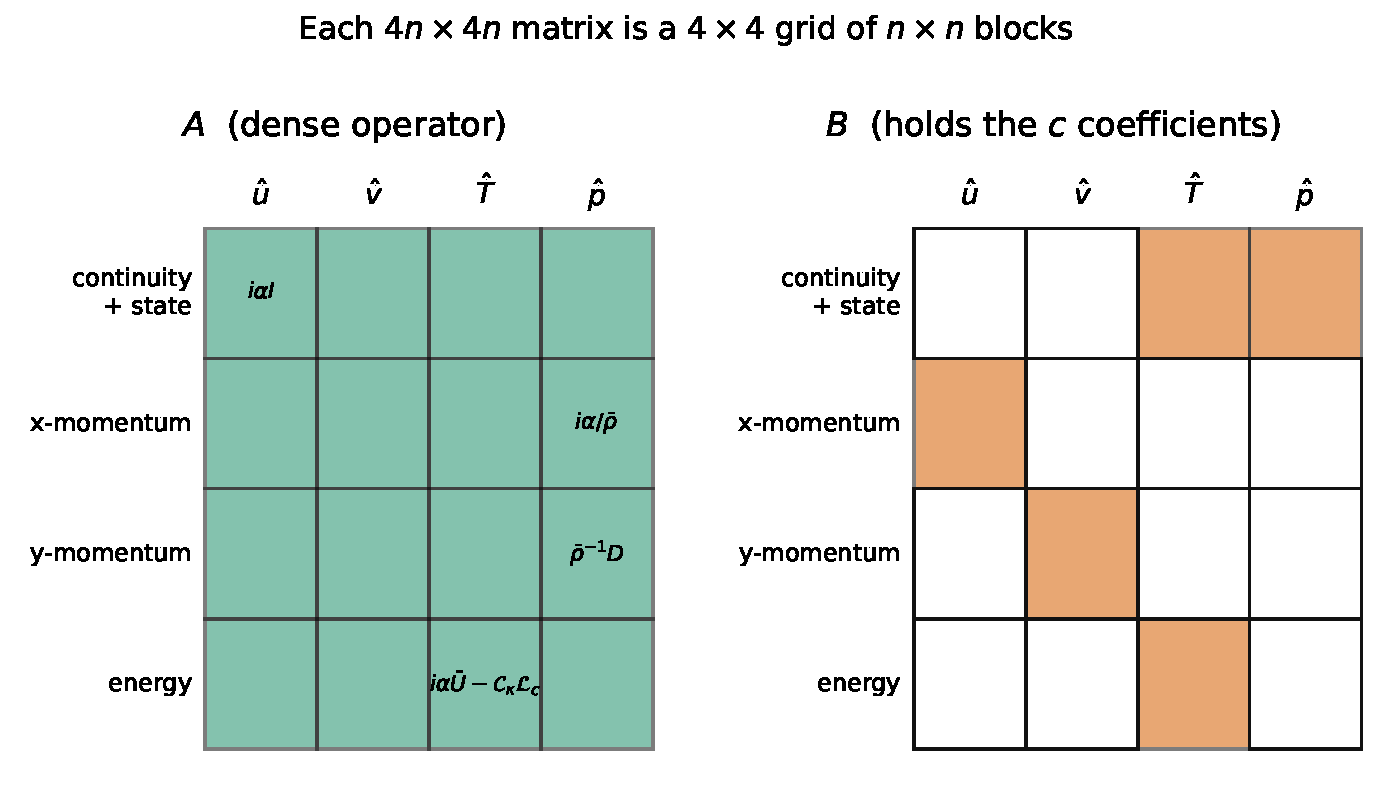
\includegraphics[width=0.95\linewidth]{fig_blocks.pdf}
  \caption{Block structure of $A\boldsymbol\phi=cB\boldsymbol\phi$. Rows: the four equations
  (continuity, $x$-momentum, $y$-momentum, energy); columns: the four fields
  $\hatu,\hatv,\hatT,\hatp$; shaded = non-zero block. $A$ (left) is block-dense; $B$ (right) holds
  only five non-zero blocks, the sparsity pattern of $\mathsf M$ in Eq.~\eqref{eq:A2M}; every
  term there carries the eigenvalue $c$.}\label{fig:blocks}
\end{figure}

\begin{figure}[H]\centering
  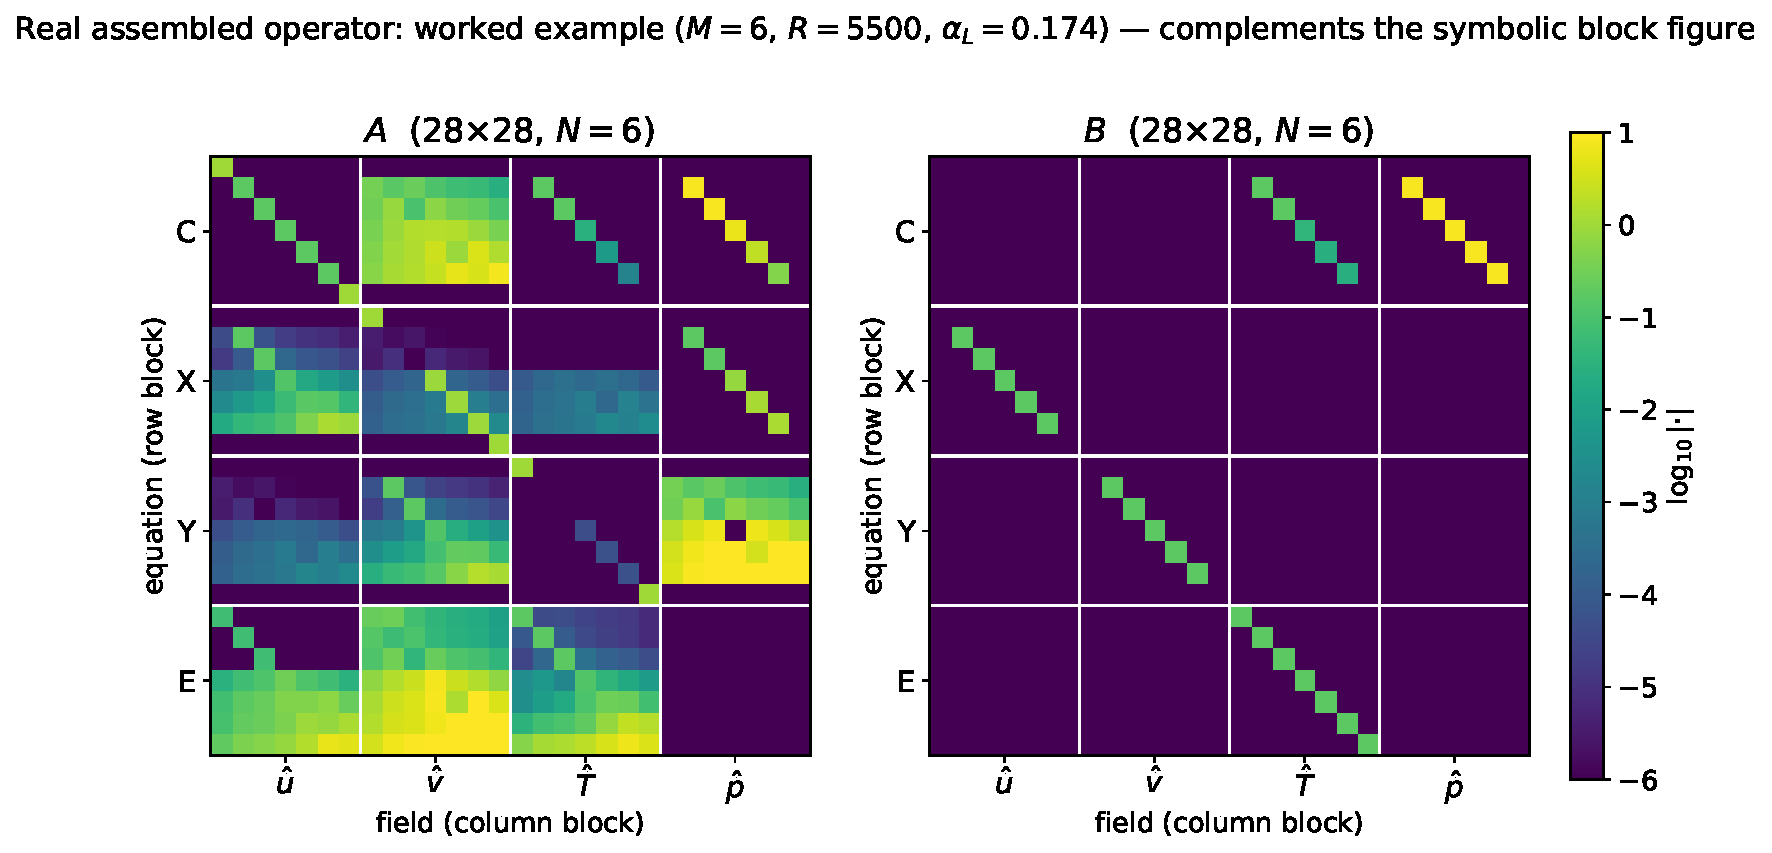
\includegraphics[width=0.95\linewidth]{fig_AB_real.pdf}
  \caption{The same block structure assembled numerically ($N=6$, $4n=28$, at the parameters of
  Section~\ref{sec:worked}), shown as $\log_{10}$ of the entry magnitudes. Gridlines every $n$
  rows/columns mark the C, X, Y, E row blocks and $\hatu,\hatv,\hatT,\hatp$ column blocks of
  Figure~\ref{fig:blocks}: $A$ is densely populated throughout, while $B$ carries only its five
  algebraic blocks.}\label{fig:ABreal}
\end{figure}

\paragraph{Boundary conditions as row replacement.} A collocation row states that the equation holds
at node $y_j$; at the wall and freestream those rows are overwritten by the boundary conditions. With
the stacking $\boldsymbol\phi=[\hatu;\hatv;\hatT;\hatp]$, field block $b\in\{0,1,2,3\}$ occupies
global indices $bn,\dots,bn+n-1$, and, from the node ordering of Section~\ref{sec:cheb}, local
index $0$ is the \emph{freestream} and local index $n{-}1$ the \emph{wall}:
\begin{center}\small
\begin{tabular}{@{}llll@{}}
\toprule
condition & field & global row & row becomes \\
\midrule
no-slip (wall)        & $\hatu$ & $n-1$    & identity ($\hatu=0$)\\
no-slip (wall)        & $\hatv$ & $2n-1$   & identity ($\hatv=0$)\\
thermal (wall)        & $\hatT$ & $3n-1$   & identity ($\hatT=0$, isothermal) \emph{or} $D_1[\text{wall},:]$ ($\D\hatT=0$, adiabatic)\\
decay (freestream)    & $\hatu$ & $0$      & identity\\
decay (freestream)    & $\hatv$ & $n$      & identity\\
decay (freestream)    & $\hatT$ & $2n$     & identity\\
\bottomrule
\end{tabular}
\end{center}
The same rows of $B$ are zeroed, so each constraint is purely algebraic; these zero rows are what
make $B$ singular and the problem irreducibly generalised. The pressure $\hatp$ carries no explicit
boundary row. The inverted node ordering is a genuine implementation hazard: because $\xi_0=+1\to
y_{\max}$ and $\xi_N=-1\to y=0$, index $0$ is the freestream and $n{-}1$ the wall, the opposite of
the naive guess, and exchanging them produces plausible-looking but wrong eigenvalues
(Figure~\ref{fig:bcrows}).

\begin{figure}[H]\centering
  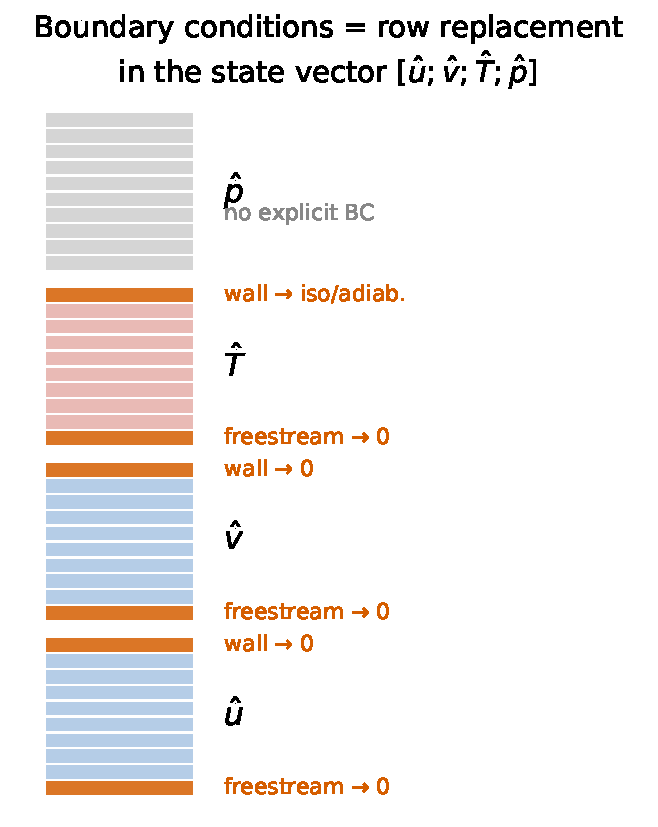
\includegraphics[width=0.45\linewidth]{fig_bc_rows.pdf}
  \caption{Boundary conditions as row replacement: the stacked state $[\hatu;\hatv;\hatT;\hatp]$ with
  the six overwritten rows highlighted (wall and freestream for $\hatu,\hatv,\hatT$); $\hatp$ carries
  no boundary row. Node index $0$ is the freestream and $n{-}1$ the wall.}\label{fig:bcrows}
\end{figure}

\section{The temporal problem: a generalised eigenvalue problem}\label{sec:temporal}
Given a real wavenumber $\alpha$, the task is to find the complex phase speed $c$ and mode shape
$\boldsymbol\phi$; the growth rate follows as $\omega_i=\alpha c_i$. With $A,B$ from
Section~\ref{sec:assemble} this is the generalised eigenvalue problem
\begin{equation}\label{eq:tEVP}
  A\boldsymbol\phi=cB\boldsymbol\phi,\qquad A,B\in\mathbb C^{4n\times4n},
\end{equation}
solved directly by the QZ algorithm \cite{molerstewart1973} (\texttt{scipy.linalg.eig}), which
returns all $4n$ eigenvalues at once; no initial guess is required, the defining advantage of the
boundary-value route \cite{malik1990}. The discrete eigenvector $\boldsymbol\phi$ is the
eigenfunction $\hatq(y)$ sampled at the grid points.

A disturbance $\propto e^{\imag\alpha(x-ct)}$ with real $\alpha$ behaves as $e^{\alpha c_it}$ in
time, so
\begin{equation}\label{eq:tgrowth}
  c_i=\Imag(c)>0\ \Rightarrow\ \text{unstable (grows in time)},\qquad c_r=\Real(c)=\text{phase speed},
\end{equation}
and the phase speed classifies the mode: a first (Tollmien--Schlichting) mode has
$c_r\approx0.3$--$0.6$, a second (Mack) mode $c_r\approx1-1/\Mae$ \cite{mack1984}. The raw spectrum
is filtered to $\Real(c)\in(-0.5,1.5)$, $|\Imag(c)|<0.5$ and sorted by $c_i$; the identification of
the physical mode within the filtered set is the subject of Section~\ref{sec:modes}.

\begin{figure}[H]\centering
  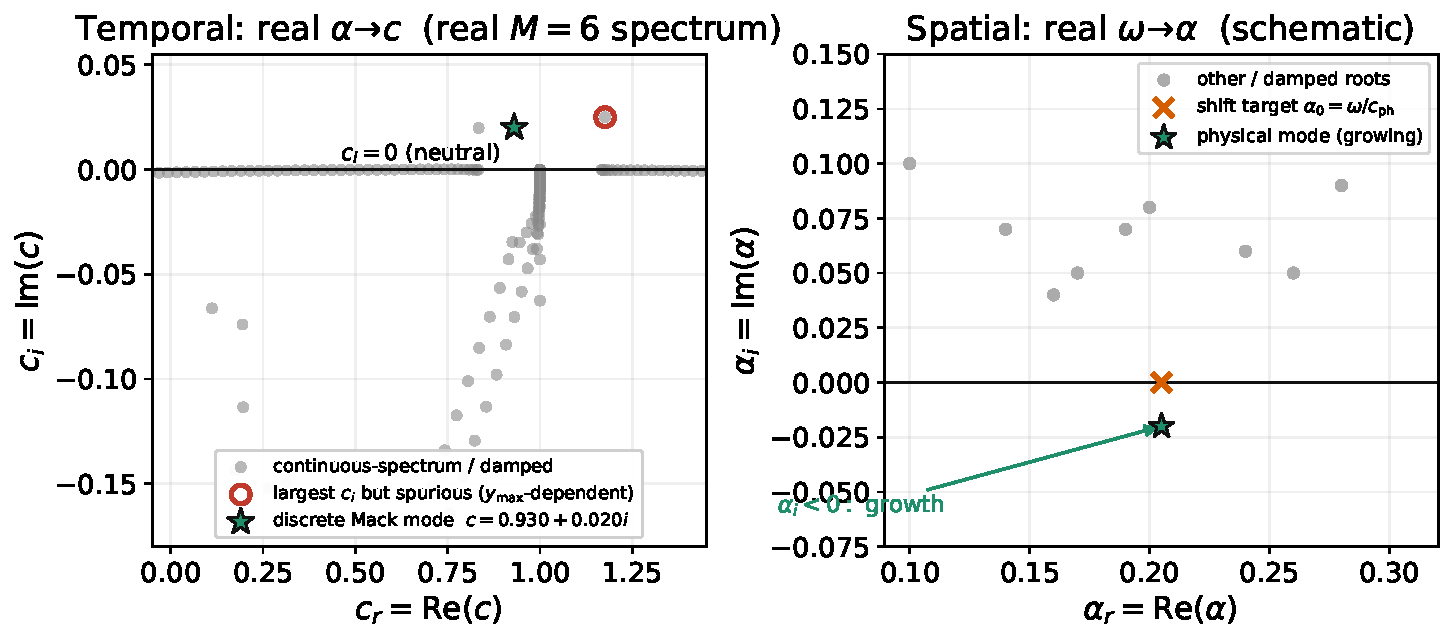
\includegraphics[width=0.95\linewidth]{fig_evp_planes.pdf}
  \caption{The two eigenvalue planes. \emph{Left (temporal):} input real $\alpha$; the phase speeds
  $c$ populate the complex plane; the physical discrete mode sits above the line $c_i=0$ (unstable)
  while the continuous spectrum is damped. \emph{Right (spatial,
  Section~\ref{sec:spatial}):} input real $\omega$; the wavenumbers $\alpha$ are sought near a shift
  target $\alpha_0$; the physical mode has $\alpha_i<0$, i.e.\ spatial growth.}\label{fig:planes}
\end{figure}

\section{The spatial problem: a quadratic eigenvalue problem}\label{sec:spatial}
Given a real frequency $\omega$ (the physically forced case, since a fixed-frequency source
generates a disturbance that grows in space), the task is to find the complex wavenumber $\alpha$;
the growth rate follows as $\sigma=-\alpha_i$. Because the viscous and conduction terms carry
$\partial_x^2\mapsto-\alpha^2$, the eigenvalue now appears quadratically. Grouping the discretised
equations by powers of $\alpha$ gives the quadratic eigenvalue problem
\begin{equation}\label{eq:qep}
  \big(C_0+\alpha C_1+\alpha^2C_2\big)\boldsymbol\phi=0 .
\end{equation}

\paragraph{The blocks $C_0,C_1,C_2$ (complete listing).} The spatial assembler (\texttt{equations.py})
uses the \emph{enthalpy} form of the energy equation, in which $\hatp$ appears explicitly through
$\D p'/\D t$ and the temperature row differs from the temporal energy row, and a bulk-viscosity
ratio $\lambda/\mu=1.2$, giving the viscous coefficients of Mack \cite[Eq.~8.5]{mack1984}
\begin{equation}\label{eq:mackcoef}
  c_{\alpha^2}=\tfrac{2(2+\lambda/\mu)}{3}=2.13,\qquad
  c_\times=\tfrac{1+2\lambda/\mu}{3}=1.13,\qquad
  c_a=\tfrac{2(\lambda/\mu-1)}{3}=0.13 .
\end{equation}
Because this closure is not obtained by re-grouping the temporal listing, all non-zero blocks are
given, transcribed from \texttt{equations.py}; $\nuR=1/(\Ree\bar\rho)$ is the viscous/conduction
prefactor and $d_R=(\gamma-1)\Mae^2\nuR$ the dissipation prefactor.
{\footnotesize
\begin{itemize}[leftmargin=2.6em,itemsep=2pt]
\item[\emph{(C)}] $C_0\!:\ \hatv\!\to D_1-\tfrac{\bar T'}{\bar T},\ \ \hatT\!\to\tfrac{\imag\omega}{\bar T},\ \ \hatp\!\to-\imag\omega\gamma\Mae^2$.\quad
  $C_1\!:\ \hatu\!\to\imag I,\ \ \hatT\!\to-\tfrac{\imag\bar U}{\bar T},\ \ \hatp\!\to\imag\gamma\Mae^2\bar U$.\quad $C_2\!:$ none.
\item[\emph{(X)}] $C_0\!:\ \hatu\!\to-\imag\omega-\nuR(\bar\mu D_2+\bar\mu'D_1),\ \ \hatv\!\to\bar U',\ \
  \hatT\!\to-\nuR\big[\tfrac{\mathrm d\mu}{\mathrm dT}(\bar U''+\bar U'D_1)+\tfrac{\mathrm d^2\mu}{\mathrm dT^2}\bar U'\bar T'\big]$.\quad
  $C_1\!:\ \hatu\!\to\imag\bar U,\ \ \hatv\!\to-\imag\nuR(c_\times\bar\mu D_1+\bar\mu'),\ \ \hatp\!\to\imag\bar\rho^{-1}$.\quad
  $C_2\!:\ \hatu\!\to c_{\alpha^2}\nuR\bar\mu$.
\item[\emph{(Y)}] $C_0\!:\ \hatv\!\to-\imag\omega-c_{\alpha^2}\nuR(\bar\mu D_2+\bar\mu'D_1),\ \ \hatp\!\to\bar\rho^{-1}D_1$.\quad
  $C_1\!:\ \hatu\!\to-\imag\nuR(c_\times\bar\mu D_1+c_a\bar\mu'),\ \ \hatv\!\to\imag\bar U,\ \ \hatT\!\to-\imag\nuR\tfrac{\mathrm d\mu}{\mathrm dT}\bar U'$.\quad
  $C_2\!:\ \hatv\!\to\nuR\bar\mu$.
\item[\emph{(E)}] $C_0\!:\ \hatu\!\to-2d_R\bar\mu\bar U'D_1,\ \ \hatv\!\to\bar T',\ \
  \hatT\!\to-\imag\omega-\nuR\big[\bar\kappa D_2+2\bar\kappa'D_1+\tfrac{\mathrm d\kappa}{\mathrm dT}\bar T''+\tfrac{\mathrm d^2\kappa}{\mathrm dT^2}(\bar T')^2\big]-d_R\tfrac{\mathrm d\mu}{\mathrm dT}(\bar U')^2,\ \ \hatp\!\to\imag\omega(\gamma-1)\Mae^2\bar\rho^{-1}$.\quad
  $C_1\!:\ \hatv\!\to-2\imag d_R\bar\mu\bar U',\ \ \hatT\!\to\imag\bar U,\ \ \hatp\!\to-\imag(\gamma-1)\Mae^2\bar U\bar\rho^{-1}$.\quad
  $C_2\!:\ \hatT\!\to\nuR\bar\kappa$.
\end{itemize}}
\noindent All other blocks are zero. The temporal closure (Stokes $\tfrac43,\tfrac13$ factors,
temperature energy row) and this spatial closure (enthalpy row, $\lambda/\mu=1.2$) differ only in the
bulk-viscosity treatment and the energy-equation arrangement; both approximate the same physical mode
and agree on it to within discretisation error.

\paragraph{Companion linearisation.} A quadratic pencil becomes an ordinary generalised problem of
twice the size by introducing the auxiliary variable $\boldsymbol\psi=\alpha\boldsymbol\phi$
\cite{tisseur2001} (\texttt{solver.py}):
\begin{equation}\label{eq:companion}
  \underbrace{\begin{bmatrix}-C_1&-C_0\\ I&0\end{bmatrix}}_{\mathcal L}
  \begin{bmatrix}\boldsymbol\psi\\ \boldsymbol\phi\end{bmatrix}
  =\alpha\,\underbrace{\begin{bmatrix}C_2&0\\ 0&I\end{bmatrix}}_{\mathcal R}
  \begin{bmatrix}\boldsymbol\psi\\ \boldsymbol\phi\end{bmatrix}.
\end{equation}
The lower block row enforces $\boldsymbol\psi=\alpha\boldsymbol\phi$; the upper row then reproduces
\eqref{eq:qep}. The eigenvalue is $\alpha$ and the physical shape is the lower half
$\boldsymbol\phi$: since $\boldsymbol\psi=\alpha\boldsymbol\phi$ the two halves are parallel, and by
convention the lower half is normalised as the eigenfunction (Figure~\ref{fig:companion}).

\begin{figure}[H]\centering
  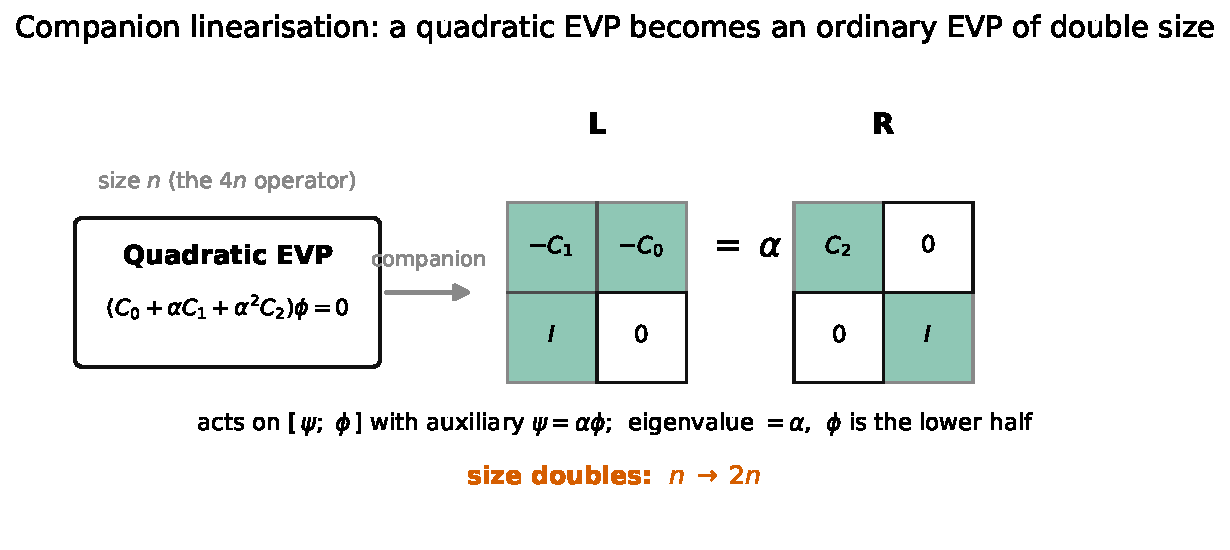
\includegraphics[width=0.9\linewidth]{fig_companion.pdf}
  \caption{Companion linearisation \eqref{eq:companion}: the $4n$-sized quadratic problem becomes an
  ordinary generalised problem of size $8n$ in $[\boldsymbol\psi;\boldsymbol\phi]$ with
  $\boldsymbol\psi=\alpha\boldsymbol\phi$. Its eigenvalue is exactly $\alpha$; the eigenfunction is
  the lower half.}\label{fig:companion}
\end{figure}

\paragraph{Shift--invert.} The physically relevant branch is targeted with a shift
$\alpha_0=\omega/c_{\mathrm{ph}}$ ($c_{\mathrm{ph}}=1-1/\Mae$ for $\Mae>3$, else $\approx0.4$;
these are the second- and first-mode phase-speed estimates of Section~\ref{sec:temporal}). Subtracting
$\alpha_0$ and inverting maps eigenvalues near $\alpha_0$ to large $\mu$:
\begin{equation}\label{eq:shift}
  \text{eigenvalues of }(\mathcal L-\alpha_0\mathcal R)^{-1}\mathcal R\ \text{ are }\ \mu=\frac1{\alpha-\alpha_0},
  \qquad\Rightarrow\qquad \alpha=\alpha_0+\frac1\mu ,
\end{equation}
so the largest-$|\mu|$ modes are the wavenumbers nearest the physical one (in \texttt{pyMack}, a
dense solve followed by selecting the $n_{\mathrm{modes}}{=}20$ eigenvalues nearest $\alpha_0$ and
sorting by $\Imag\alpha$). The amplitude varies as
$e^{\imag\alpha x}=e^{\imag\alpha_rx}e^{-\alpha_ix}$, so
\begin{equation}\label{eq:sgrowth}
  \sigma=-\Imag(\alpha)=-\alpha_i>0\ \Rightarrow\ \text{unstable (grows downstream)}.
\end{equation}

\paragraph{Alternative route: Newton iteration from a temporal seed.} When shift--invert struggles, a
more robust path (\texttt{solve\_spatial\_from\_temporal}) solves the \emph{temporal} problem at a
real trial wavenumber $\alpha_r=\omega/c_{\mathrm{est}}$ ($c_{\mathrm{est}}=0.98$ for $\Mae>3$, else
$0.35$), keeping only modes that agree across two resolutions (tolerance $8\times10^{-3}$); forms the
seed $\Imag(\alpha)\approx-\alpha_rc_i/c_r$, a phase-speed estimate of the rigorous
group-velocity conversion of Gaster \cite{gaster1962} that suffices here because it only seeds the
iteration, and then Newton-iterates the dispersion residual $F(\alpha)=\alpha c(\alpha)-\omega=0$,
$\alpha^{(k+1)}=\alpha^{(k)}-F/F'$, with $F'$ approximated by a finite difference (step $10^{-5}$,
tolerance $10^{-6}$, at most $20$ iterations). Both routes return the same $\sigma=-\alpha_i$.

\section{Identifying the physical mode}\label{sec:modes}
A single solve of \eqref{eq:tEVP} returns $4n$ eigenvalues, of which only a handful are genuine
boundary-layer modes; the task is to select them. Besides the discrete modes, the operator possesses
a \emph{continuous spectrum}: on an unbounded domain the freestream solutions form a continuous
band rather than isolated points, which the finite grid renders as a dense cluster of spurious
discrete eigenvalues. Two tests (\texttt{discrete\_mode.py}) separate the physical mode:
\begin{enumerate}[nosep,leftmargin=1.8em]
  \item \textbf{Freestream decay.} A true boundary-layer eigenfunction decays as $y\to y_{\max}$; a
        continuous-spectrum mode oscillates undiminished to the edge. Candidates whose edge-to-peak
        amplitude ratio exceeds ${\sim}0.06$ are rejected.
  \item \textbf{Domain stationarity.} A genuine eigenvalue is insensitive to the truncation height.
        The solve is repeated at two domain heights and only modes whose $c$ matches to
        ${\sim}4\times10^{-3}$ are kept; accepted growth rates additionally satisfy
        $|c_i|\lesssim0.05$ with $c_r$ in the physical band.
\end{enumerate}
These two tests are what allow a single trusted number to be extracted from the full spectrum; the
worked example below shows why they are indispensable: its largest-growth eigenvalue is in fact
spurious.

\section{Worked example: one temporal solve}\label{sec:worked}
Consider a strong Mack-mode case: $\Mae=6.0$, $R=5500$, $\alpha_L=0.174$, adiabatic wall, $L^*$
scaling, $N=180$ ($n=181$, matrices $4n=724$ wide), and domain height
$y_{\max}=10\,(\delta^*/L^*)\approx128$ (a multiple of the boundary-layer scale, per
Section~\ref{sec:cheb}). Solving \eqref{eq:tEVP} returns $724$ eigenvalues; after the physical
filter, the six least-stable are:
\begin{center}\small
\begin{tabular}{@{}rrrll@{}}
\toprule
$c_r$ & $c_i$ & $\omega_i=\alpha c_i$ & $y_{\max}$-stationary? & verdict \\
\midrule
$+1.176$ & $+0.0249$ & $+0.00434$ & no ($|\Delta c|\!\sim\!10^{-2}$) & spurious / continuous spectrum \\
$\mathbf{+0.930}$ & $\mathbf{+0.0200}$ & $\mathbf{+0.00348}$ & \textbf{yes} ($|\Delta c|\!\sim\!10^{-7}$) & \textbf{discrete Mack mode (the answer)} \\
$+0.834$ & $+0.0197$ & $+0.00343$ & no & continuous spectrum \\
$+0.740$ & $+0.0000$ & $\phantom{+}0.00000$ & n/a & neutral continuous-spectrum cluster \\
$+0.720$ & $+0.0000$ & $\phantom{+}0.00000$ & n/a & continuous spectrum \\
$+0.760$ & $+0.0000$ & $\phantom{+}0.00000$ & yes & stable discrete mode \\
\bottomrule
\end{tabular}
\end{center}
This is precisely the trap the tests of Section~\ref{sec:modes} exist to avoid: the largest-growth
eigenvalue (first row, $c_r=1.18$) is \emph{not} the answer: its $c$ shifts by ${\sim}10^{-2}$
when the domain height changes, and $c_r>1$ is unphysically supersonic. The physical answer is the
second row, the Mack (second) mode $c=0.930+0.0200\imag$: domain-stationary to $10^{-7}$, with an
eigenfunction that decays at the freestream (Figure~\ref{fig:eigfn}). Its growth rate is
$\omega_i=\alpha c_i=+0.00348$ (unstable) and its phase speed $c_r=0.93$ is the second-mode value
near $1-1/\Mae$ \cite{mack1984}. This single $\omega_i>0$ is one point inside the neutral curve;
repeating the solve across an $(R,\alpha)$ grid and locating the zero crossing of $\omega_i$ traces
the neutral curve of Section~\ref{sec:neutral}. All numbers reproduce from
\texttt{solve\_temporal\_2d}.

\begin{figure}[H]\centering
  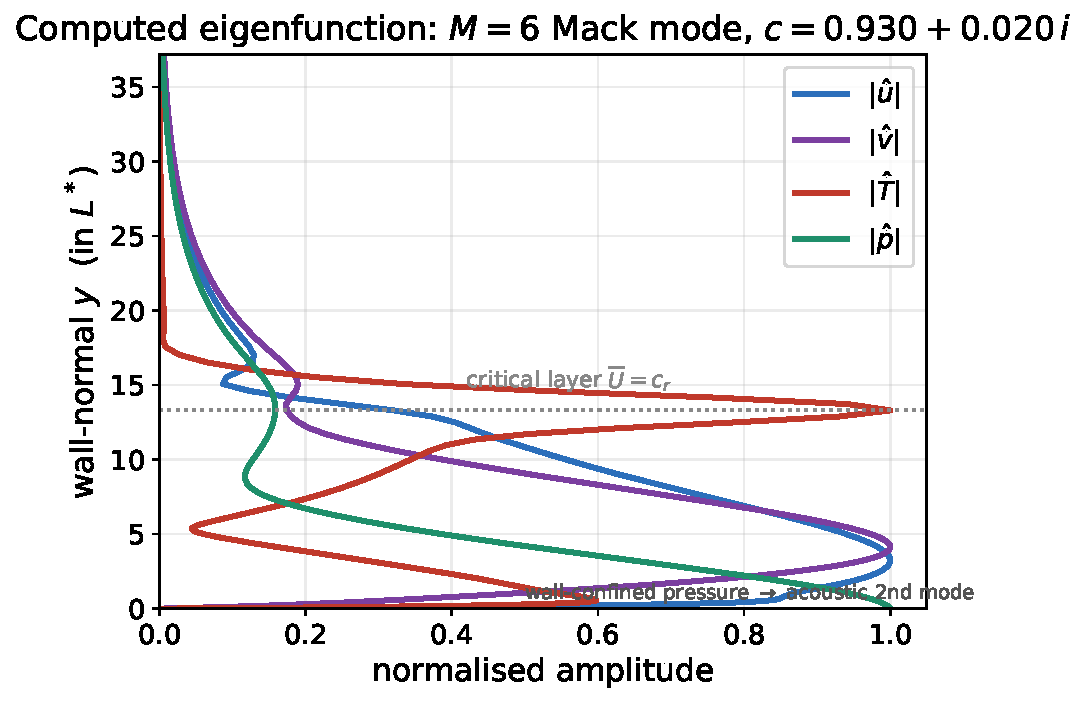
\includegraphics[width=0.58\linewidth]{fig_eigenfunctions.pdf}
  \caption{Computed eigenfunction of the worked-example Mack mode: the four amplitude fields
  $|\hatu|,|\hatv|,|\hatT|,|\hatp|$ against $y$ (each normalised). $|\hatT|$ peaks at the critical
  layer ($\bar U=c_r$); $|\hatp|$ is wall-confined, the acoustic signature of the second mode. All
  fields decay at the freestream, confirming a discrete mode.}\label{fig:eigfn}
\end{figure}

\section{Neutral curves}\label{sec:neutral}
The neutral curve is the boundary between growth and decay: the locus $c_i(R,\alpha)=0$ (temporal) or
$\sigma(R,\omega)=0$ (spatial), inside which the flow is unstable. \texttt{pyMack} traces it in three
steps:
\begin{enumerate}[nosep,leftmargin=1.8em]
  \item \textbf{Sweep} an $(R,\alpha)$ grid at fixed $\Mae$; at each node solve \eqref{eq:tEVP},
        apply the mode tests of Section~\ref{sec:modes}, and store $c_i$
        (\texttt{build\_*\_grid.py}).
  \item \textbf{Extract} the zero contour of the stored field by marching squares
        (\texttt{extract\_contours.py}); unresolved nodes are tagged stable so that the contour
        closes.
  \item \textbf{Continuation} for difficult branches: at low Mach number the first-mode eigenvalue
        approaches the continuous spectrum and the grid sweep loses it.
        \texttt{trace\_continuation.py} tracks the mode by proximity: from a clean seed it marches
        in $R$, follows the nearest eigenvalue, and secant-solves $c_i=0$ at each step, each
        converged eigenvalue seeding the next parameter value.
\end{enumerate}

\begin{figure}[H]\centering
  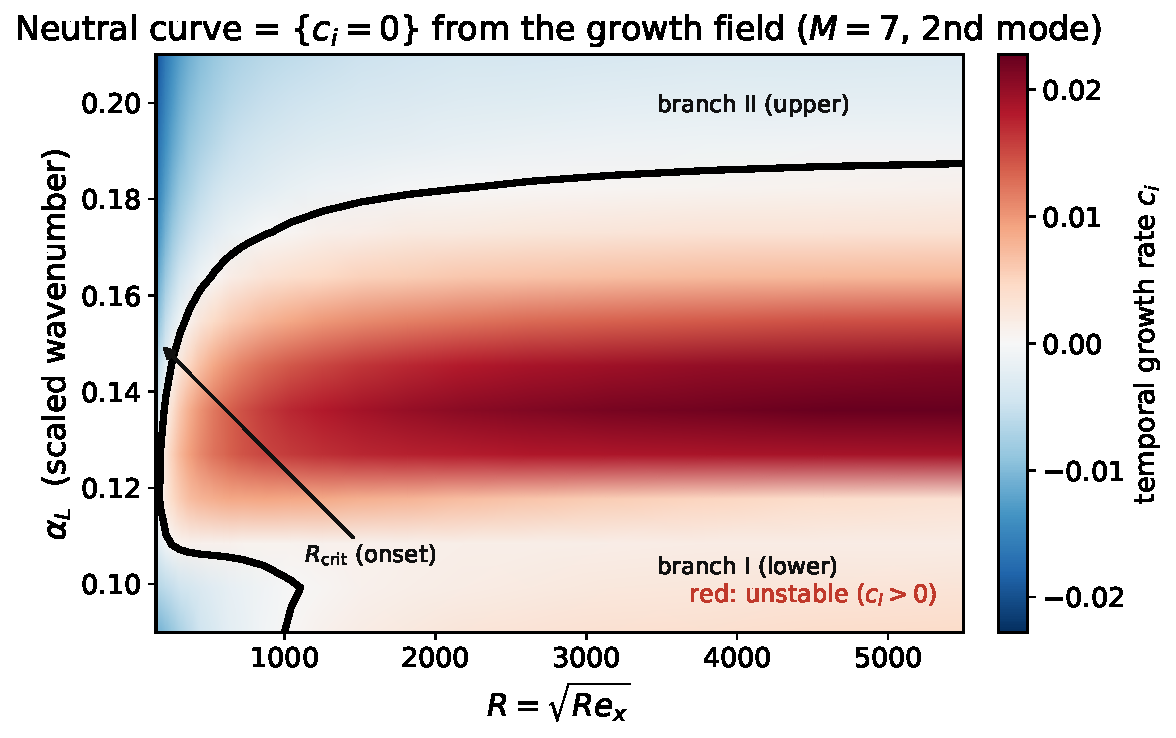
\includegraphics[width=0.85\linewidth]{fig_neutral_field.pdf}
  \caption{Steps 1--2 of the neutral-curve procedure for a solved case ($\Mae=7$, second mode): the
  coloured field is the growth rate $c_i(R,\alpha)$ from the sweep; the black curve is the extracted
  $\{c_i=0\}$ contour. The flow is unstable inside the loop; $R_{\mathrm{crit}}$ marks the lower
  branch (branch~I) where instability first appears as $R$ increases, and the curve closes at
  branch~II.}\label{fig:neutral}
\end{figure}

\section{$N$-factor and transition}\label{sec:nfactor}
What matters for transition is the \emph{accumulated} amplification of a fixed-frequency disturbance.
For a chosen reduced frequency $F$, the spatial problem of Section~\ref{sec:spatial} is solved at
successive stations to obtain $\sigma_L=-\Imag(\alpha_L)$, the spatial growth rate
\eqref{eq:sgrowth} expressed in the $L^*$ scaling, and integrated from the lower neutral point
$R_0$ where $\sigma_L$ first becomes positive:
\begin{equation}\label{eq:N}
  N(R)=\int_{R_0}^R\max(\sigma_L,0)\,\mathrm dR'\quad\text{(trapezoidal)},\qquad
  \frac{A(R)}{A(R_0)}=e^{N(R)} .
\end{equation}
The amplitude grows by $e^N$, and transition is empirically expected near $N\approx9$--$11$,
following the $e^N$ method of Smith \& Gamberoni and van Ingen \cite{smith1956,vaningen1956}
(\texttt{analysis.py}). For a cone, surface arc length is mapped to an equivalent $R$ before
integration. The transition $N$ is a correlation, not a first-principles criterion: it depends on the
disturbance environment (flight ${\sim}9$--$11$; noisy conventional tunnels transition at
$N\sim4$--$6$), presumes a single dominant linear mode, and absorbs the unknown initial amplitude
set by receptivity.

\begin{figure}[H]\centering
  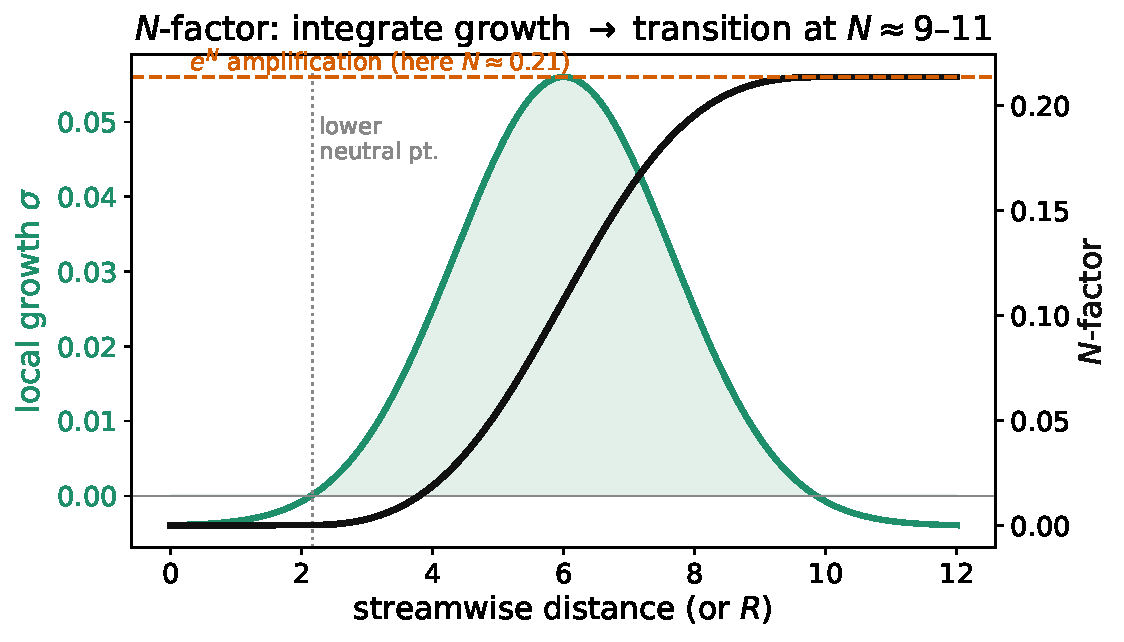
\includegraphics[width=0.85\linewidth]{fig_nfactor.pdf}
  \caption{The $N$-factor integration, Eq.~\eqref{eq:N}: the shaded area is $\max(\sigma_L,0)$, the
  local spatial growth carried from station to station; the black curve is the running integral
  $N(R)$. The growth-rate curve is schematic (a rescaled synthetic $\sigma_L(R)$), drawn to reach the
  empirical transition band $N\approx9$--$11$ so the asymptote can be read against that
  criterion.}\label{fig:nfactor}
\end{figure}

\section{Part A summary and replication checklist}\label{sec:summary}
\begin{center}\small
\renewcommand{\arraystretch}{1.25}
\begin{tabular}{@{}>{\raggedright\arraybackslash}p{2.7cm}>{\raggedright\arraybackslash}p{4.6cm}
>{\raggedright\arraybackslash}p{4.4cm}>{\raggedright\arraybackslash}p{2.4cm}@{}}
\toprule
\textbf{Goal} & \textbf{Problem solved} & \textbf{Method} & \textbf{Growth} \\
\midrule
Temporal growth, neutral curves
  & generalised EVP $A\boldsymbol\phi=cB\boldsymbol\phi$, real $\alpha$ (Eq.~\ref{eq:tEVP})
  & Chebyshev collocation $+$ QZ & $\alpha c_i$ \\
Spatial growth, $N$-factor
  & quadratic EVP $(C_0+\alpha C_1+\alpha^2C_2)\boldsymbol\phi=0$, real $\omega$ (Eq.~\ref{eq:qep})
  & companion $+$ shift--invert; or temporal $+$ Newton seed & $-\alpha_i$ \\
Neutral curve
  & $\{c_i=0\}$ over an $(R,\alpha)$ sweep (Figure~\ref{fig:neutral})
  & grid sweep $\to$ marching squares; continuation & n/a \\
Transition
  & $N=\int\max(\sigma_L,0)\,\mathrm dR$ (Eq.~\ref{eq:N}, Figure~\ref{fig:nfactor})
  & fixed-$F$ spatial march $+$ integration & n/a \\
\bottomrule
\end{tabular}
\end{center}

\paragraph{To re-implement the spectral solver from scratch.}
\begin{enumerate}[nosep,leftmargin=1.9em]
  \item Solve the base-flow boundary-value problem (companion \emph{Mean Boundary-Layer} document);
        tabulate $\bar U,\bar T$ and derivatives.
  \item Build $\xi_j$ \eqref{eq:gll}, $D_\xi$ \eqref{eq:Dformula}, map to $y$ \eqref{eq:map}, form
        $D_1,D_2$ \eqref{eq:Dmats}.
  \item Assemble the $4\times4$ block operator (temporal: the coefficient matrices
        \eqref{eq:A2M}--\eqref{eq:A0} via the assembly rule \eqref{eq:assembly}; spatial:
        $C_0,C_1,C_2$).
  \item Overwrite the wall/freestream rows with the boundary conditions
        (Section~\ref{sec:assemble}), respecting the node ordering.
  \item Solve the eigenvalue problem (temporal \eqref{eq:tEVP} or spatial \eqref{eq:companion});
        filter for the discrete mode (Section~\ref{sec:modes}); read $c_i$ or $-\alpha_i$.
  \item Sweep parameters; extract $\{c_i=0\}$ for neutral curves, or integrate $-\alpha_i$ for
        $N$-factors.
\end{enumerate}

\bigskip
{\sloppy
\noindent\emph{Code map (Part~A).} spectral operators: \texttt{pymack/\allowbreak spectral.py};
temporal assembly: \texttt{pymack/\allowbreak temporal\_solver.py}; spatial assembly:
\texttt{pymack/\allowbreak equations.py}; solvers / companion / Newton:
\texttt{pymack/\allowbreak solver.py}; mode selection: \texttt{discrete\_mode.py}. Neutral-curve
drivers and continuation: \texttt{build\_*\_grid.py}, \texttt{extract\_contours.py},
\texttt{trace\_\allowbreak continuation.py}.
\par}

%=====================================================================
\part*{Part B: The shooting solver}
\addcontentsline{toc}{section}{Part B: The shooting solver}
%=====================================================================
Part~A built one large matrix and asked a dense eigensolver for all of its eigenvalues. Part~B poses
the identical temporal question (for a given real $\alpha$, at what complex $c$ does a non-trivial
disturbance satisfy decay at the freestream and the wall conditions?) as an \emph{initial-value}
computation \cite{malik1990}: the disturbance equations are recast as a small first-order system,
integrated from the freestream to the wall, and the eigenvalue is located by driving a $3\times3$
wall matrix singular. No global matrix is ever formed; the cost per evaluation is small, but a good
initial guess is required. This is the classical shooting procedure of Mack \cite{mack1984},
implemented in \texttt{pymack/\allowbreak temporal\_shooting.py} in the formulation of \"Ozgen \&
K{\i}rcal{\i} \cite{ozgen2008}. Within \texttt{pyMack} its role is verification and refinement: given
a mode located by the spectral solver, shooting confirms it through entirely independent numerics and
sharpens it to tight tolerance. Figure~\ref{fig:shooting} shows the complete pipeline.

\begin{figure}[H]\centering
  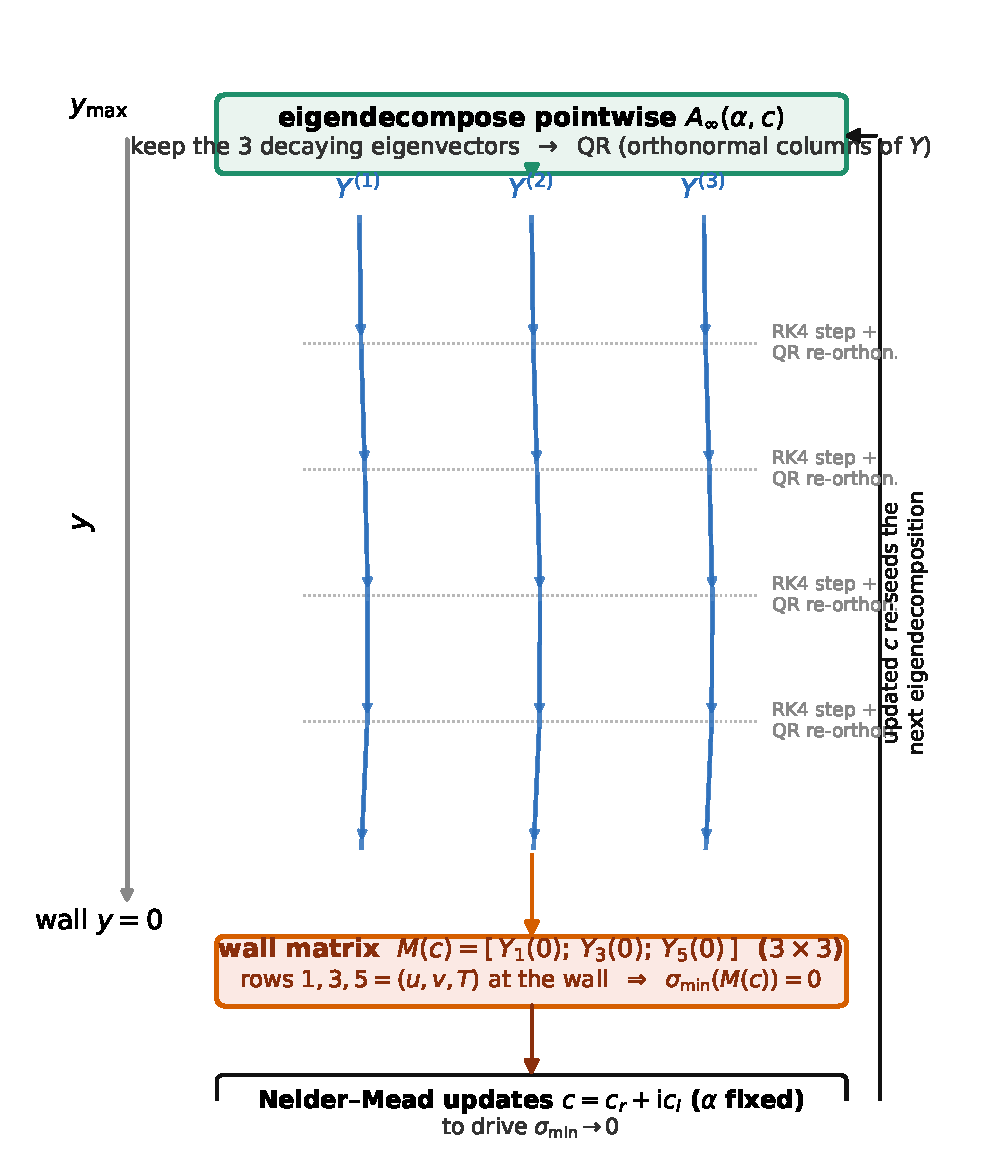
\includegraphics[width=0.92\linewidth]{fig_shooting_scheme.pdf}
  \caption{The shooting pipeline, top ($y_{\max}$) to bottom (wall, $y=0$). At $y_{\max}$ the
  constant-coefficient matrix $A_\infty$ is eigen-decomposed and its three decaying eigenvectors are
  QR-orthonormalised into the starting $6\times3$ basis (Section~\ref{sec:shoot-bc}); the basis is
  RK4-marched to the wall with re-orthonormalisation after every step
  (Section~\ref{sec:shoot-integrate}); at the wall the three arriving columns form the $3\times3$
  matrix $M(c)$ (Section~\ref{sec:shoot-wall}); and an outer Nelder--Mead loop
  (Section~\ref{sec:shoot-search}) updates the trial $c$ to drive $\sigma_{\min}(c)\to0$, feeding
  back into the eigen-decomposition at $y_{\max}$.}\label{fig:shooting}
\end{figure}

\section{The first-order state and its coefficient matrix}\label{sec:shoot-system}
Given a real wavenumber $\alpha$ and a trial phase speed $c$, the four disturbance equations are cast
as a single first-order ODE in a six-component complex state. Following \"Ozgen \& K{\i}rcal{\i}
\cite[Eqs.~22--28]{ozgen2008}, specialised to two dimensions ($\beta=0$, no spanwise velocity), the
state is
\begin{equation}\label{eq:state}
  Y(y)=\big(X_1,X_2,X_3,X_4,X_5,X_6\big)^{\mathsf T}\in\mathbb C^{6},
\end{equation}
in which $X_1,X_3,X_5$ are the primary flow amplitudes, $X_2,X_6$ the wall-normal derivatives of
$X_1,X_5$, and $X_4$ the pressure amplitude. Concretely, $X_1=\alpha\hatu$ is the wavenumber-scaled
streamwise-velocity amplitude (the $k$-direction combination $\alpha\hat u+\beta\hat w$ of
\cite{ozgen2008} evaluated at $\beta=0$; the constant factor $\alpha$ is immaterial in a homogeneous
eigenvalue problem), $X_3=\hatv$ the wall-normal velocity, $X_5=\hatT$ the temperature (with
$X_2=\D X_1$, $X_6=\D X_5$), and $X_4=\hatp$ the same $\rho_eU_e^2$-scaled pressure as Part~A,
coupled through the continuity and $y$-momentum rows rather than as a plain derivative. The state
thus stacks $(\alpha u,\ \alpha u',\ v,\ p,\ T,\ T')$, and the system closes as one first-order ODE,
\begin{equation}\label{eq:foode}
  \frac{\mathrm d Y}{\mathrm d y}=A\big(y;\ \alpha,c,\Ree,\Mae\big)\,Y,\qquad A\in\mathbb C^{6\times6},
\end{equation}
where $A$ is assembled \emph{pointwise}, one $6\times6$ matrix at each $y$, from the local
mean-flow data $\bar U,\bar U',\bar U''$, $\bar T,\bar T'$, $\bar\mu$ with
$\mathrm d\mu/\mathrm dT,\ \mathrm d^2\mu/\mathrm dT^2$, and $\bar\kappa$ with its temperature
derivatives (function \texttt{ozgen\_\allowbreak first\_order\_\allowbreak matrix\_2d}). Rows $1$
and $5$ of $A$ carry the trivial derivative definitions $\D X_1=X_2$ and $\D X_5=X_6$ (single
entries $A_{12}=A_{56}=1$); the physics resides in rows $2,4,6$ (the two momentum balances and the
energy balance) and in row $3$, continuity with the equation of state.

The pointwise structure mirrors the block operator of Part~A term for term: the convective factor
$\alpha(\bar U-c)$, the viscous prefactor $\propto\Ree/(\bar\mu\bar T)$, the transport-derivative
couplings $\tfrac{\mathrm d\mu}{\mathrm dT}\bar U'$, and the conduction group in $\bar\kappa$ all
reappear, now as scalar entries of a $6\times6$ matrix at one height rather than as $n\times n$
blocks. The gas defaults ($\gamma=1.4$) and the length scaling (\texttt{L\_star}) match the spectral
solver, so both routes see the identical mean flow.

\paragraph{Remark: single source of truth, and a correction to the printed reference.} Internally,
\texttt{ozgen\_first\_order\_matrix\_2d} delegates to the Mack Appendix-A matrix
(\texttt{mack\_shooting.mack\_first\_order\_matrix\_6}) evaluated at $\beta=0$ with $\lambda/\mu=0$
(the same Stokes closure as Part~A's temporal solver), which at those settings is algebraically
identical to the printed Eqs.~22--28 of \cite{ozgen2008}, term for term, with one correction: the
$X_1$ coefficient of the printed Eq.~(24) reads
$+\imag\big(2\mu\tfrac{\mathrm d\mu}{\mathrm dT}T'+\tfrac43\tfrac{T'}{T}\big)$, but re-deriving the
pressure row from Eqs.~(13) and (23) of the same reference gives
$-\imag\big(2\tfrac1\mu\tfrac{\mathrm d\mu}{\mathrm dT}T'+\tfrac43\tfrac{T'}{T}\big)$ (sign and
$\mu$-placement). With the corrected term the two solvers agree in practice: at the worked-example
parameters of Section~\ref{sec:worked}, $\sigma_{\min}(c)$ falls to $4\times10^{-6}$ at the spectral
eigenvalue $c=0.930+0.0200\imag$ and rises by two orders of magnitude within
$|\Delta c|\sim2\times10^{-3}$ of it.

\section{Boundary conditions: the wall and the decaying freestream basis}\label{sec:shoot-bc}
Six conditions pin down a non-trivial disturbance: three homogeneous conditions at the wall, and
three at the freestream selecting only the decaying solutions.

\paragraph{Wall conditions.} At $y=0$ the three primary amplitudes vanish,
\begin{equation}\label{eq:wallbc}
  X_1(0)=0\ \text{(no slip)},\qquad X_3(0)=0\ \text{(no penetration)},\qquad
  X_5(0)=0\ \text{(isothermal wall)},
\end{equation}
the pointwise counterparts of the spectral solver's wall identity rows
(Section~\ref{sec:assemble}).

\paragraph{Freestream: the decaying basis.} As $y\to y_{\max}$ the mean flow becomes uniform and the
coefficient matrix approaches a constant, $A_\infty=A(y_{\max})$. A constant-coefficient system
$\D Y=A_\infty Y$ has solutions $Y\propto e^{\lambda y}v$ built from the eigenpairs $(\lambda,v)$ of
$A_\infty$; the six eigenvalues split into three with $\Real\lambda>0$, which grow outward and are
unphysical, and three with $\Real\lambda<0$, which decay outward as a bounded mode requires. Only the
three decaying eigenvectors are retained (function
\texttt{ozgen\_freestream\_decay\_basis\_2d}),
\begin{equation}\label{eq:decay}
  A_\infty v_k=\lambda_k v_k,\qquad \Real(\lambda_k)<0,\quad k=1,2,3,
\end{equation}
assembled into a $6\times3$ matrix and orthonormalised by a QR factorisation into the starting basis
$Y(y_{\max})$. Enforcing decay in this way is the shooting analogue of the spectral solver's
freestream identity rows. If a trial $c$ yields fewer than three strictly decaying eigenvalues, the
code takes the three most decaying (smallest $\Real\lambda$) so the march remains well defined; near
the physical eigenvalue exactly three decay.

\section{Integrating the bounded basis to the wall}\label{sec:shoot-integrate}
The three admissible freestream solutions must be propagated to the wall so their arrival values can
be tested against \eqref{eq:wallbc}. Because three independent solutions are tracked simultaneously,
the state is the $6\times3$ matrix $Y$ whose columns are the three solutions. It is marched from
$y_{\max}$ down to $y=0$ on a fixed grid of about $n_{\text{steps}}=800$ steps with the classical
fourth-order Runge--Kutta scheme (function \texttt{integrate\_ozgen\_bounded\_basis\_2d}); over one
step of size $h$ (here $h<0$),
\begin{equation}\label{eq:rk4}
\begin{aligned}
  k_1&=A(y_0)\,Y, & k_2&=A(y_m)\big(Y+\tfrac12 h\,k_1\big), \\
  k_3&=A(y_m)\big(Y+\tfrac12 h\,k_2\big), & k_4&=A(y_1)\big(Y+h\,k_3\big),
\end{aligned}
\qquad
Y\leftarrow Y+\frac{h}{6}\big(k_1+2k_2+2k_3+k_4\big),
\end{equation}
with $y_m=\tfrac12(y_0+y_1)$ the step midpoint and $A(\cdot)$ the pointwise matrix of
Section~\ref{sec:shoot-system}.

\paragraph{Re-orthonormalisation.} The three solutions decay at very different rates, so after a
short march the rapidly decaying columns are numerically swamped by the slowest one and the basis
collapses toward a single direction, the parasitic-error pathology classical in shooting for stiff
stability problems \cite{conte1966,mack1984}. To suppress it, after every RK4 step the columns are
re-orthonormalised by a QR factorisation,
\begin{equation}\label{eq:reortho}
  Y\ \longleftarrow\ Q,\qquad\text{where}\quad Y=QR\ \ (Q\in\mathbb C^{6\times3}\ \text{orthonormal}),
\end{equation}
retaining only the orthonormal factor; the discarded triangular factor merely records scaling. The
operation preserves the \emph{subspace} spanned by the columns while keeping them well conditioned,
and it is that subspace, not the individual column magnitudes, on which the eigenvalue
condition below depends.

\section{The eigenvalue condition and the wall matrix}\label{sec:shoot-wall}
At the wall the integrated basis is a $6\times3$ matrix $Y(0)$, and any admissible disturbance is a
combination $Y(0)\,a$ of its columns, $a\in\mathbb C^3$. The wall conditions \eqref{eq:wallbc}
require rows $1,3,5$ of that combination to vanish; collecting those rows gives the $3\times3$
\emph{wall matrix} (function \texttt{ozgen\_temporal\_wall\_matrix\_2d})
\begin{equation}\label{eq:wallmat}
  M(c)=\begin{bmatrix} Y_{1}(0)\\ Y_{3}(0)\\ Y_{5}(0)\end{bmatrix}\in\mathbb C^{3\times3},
  \qquad\text{wall conditions:}\quad M(c)\,a=0 .
\end{equation}
A non-trivial $a\neq0$ exists only when $M(c)$ is singular. Rather than testing a determinant, which
is poorly scaled after the repeated re-orthonormalisation, the code monitors the smallest singular
value of $M(c)$ (function \texttt{ozgen\_temporal\_sigma\_min\_2d}),
\begin{equation}\label{eq:sigmamin}
  \sigma_{\min}(c)=\min\operatorname{svd}\!\big(M(c)\big),\qquad
  \boxed{\,\sigma_{\min}(c)\to0\ \Longleftrightarrow\ c\ \text{is an eigenvalue}\,},
\end{equation}
a non-negative, well-scaled measure of distance to singularity: it vanishes exactly when the three
decaying solutions can be combined to satisfy all three wall conditions, that is, exactly when a
genuine boundary-layer mode exists at that $c$.

\section{The eigenvalue search}\label{sec:shoot-search}
It remains to locate the complex $c=c_r+\imag c_i$ at which $\sigma_{\min}(c)=0$, starting from a
physics-based guess; this single $c$ is the temporal eigenvalue, identical to the one Part~A
returns. Since $c$ is complex, driving $\sigma_{\min}\to0$ is a two-dimensional real minimisation
over $(c_r,c_i)$. \texttt{pyMack} applies the Nelder--Mead simplex method \cite{neldermead1965}
(\texttt{scipy.optimize.minimize}, function
\texttt{solve\_\allowbreak ozgen\_\allowbreak temporal\_\allowbreak mode\_2d\_\allowbreak sigma\_min})
to the objective $\sigma_{\min}$, from an initial guess such as the second-mode estimate
$c_r\approx1-1/\Mae$. The search is confined to the physical strip
\begin{equation}\label{eq:bounds}
  c_r\in(0,\,1.2),\qquad c_i\in(-0.2,\,0.2),
\end{equation}
enforced by a large penalty ($10^{6}$) outside the box, and converges to the tolerances
\begin{equation}\label{eq:tols}
  \texttt{xatol}=10^{-7}\ (\text{in }c),\qquad \texttt{fatol}=10^{-8}\ (\text{in }\sigma_{\min}),
\end{equation}
within at most ${\sim}120$ iterations. Each objective evaluation runs the entire pipeline of
Sections~\ref{sec:shoot-bc}--\ref{sec:shoot-wall} (Figure~\ref{fig:shooting}): build the freestream
decay basis, integrate with re-orthonormalisation to the wall, form $M(c)$, take $\sigma_{\min}$.
The converged minimiser is the eigenvalue, and the growth rate follows exactly as in Part~A,
$\omega_i=\alpha c_i$. The five stages map to functions as follows:

\begin{center}\footnotesize
\renewcommand{\arraystretch}{1.3}
\begin{tabular}{@{}r>{\raggedright\arraybackslash}p{5.5cm}>{\raggedright\arraybackslash}p{6.2cm}@{}}
\toprule
step & operation & function \\
\midrule
1 & build the $6\times6$ pointwise matrix $A(y)$ from the mean flow & \texttt{ozgen\_first\_order\_matrix\_2d} \\
2 & eigen-decompose $A(y_{\max})$; keep the 3 decaying modes; QR to a $6\times3$ basis & \texttt{ozgen\_freestream\_decay\_basis\_2d} \\
3 & RK4-march the $6\times3$ basis $y_{\max}\!\to\!0$, QR after every step & \texttt{integrate\_ozgen\_bounded\_basis\_2d} \\
4 & collect wall rows $(X_1,X_3,X_5)$ into $M(c)$; take $\sigma_{\min}(c)$ & \texttt{ozgen\_temporal\_wall\_matrix\_2d}, \texttt{ozgen\_temporal\_sigma\_min\_2d} \\
5 & Nelder--Mead over $(c_r,c_i)$ until $\sigma_{\min}\!\to\!0$; return $c$ & \texttt{solve\_ozgen\_temporal\_mode\_2d\_sigma\_min} \\
\bottomrule
\end{tabular}
\end{center}

\section{Spectral versus shooting}\label{sec:shoot-compare}
The two solvers answer the identical question (for a given real $\alpha$, at what complex $c$ does
a non-trivial disturbance decay at the freestream and satisfy the wall conditions?) and return the
same physical phase speed, but with complementary characteristics, mirroring the classical
boundary-value/initial-value trade-off \cite{malik1990}:

\begin{center}\small
\renewcommand{\arraystretch}{1.28}
\begin{tabular}{@{}>{\raggedright\arraybackslash}p{3.0cm}>{\raggedright\arraybackslash}p{5.2cm}>{\raggedright\arraybackslash}p{5.2cm}@{}}
\toprule
 & \textbf{Spectral (Part~A)} & \textbf{Shooting (Part~B)} \\
\midrule
core object & one $4n\times4n$ pair $(A,B)$ & one $6\times6$ matrix $A(y)$, evaluated pointwise \\
what it returns & \emph{all} $4n$ eigenvalues at once & \emph{one} eigenvalue near a guess \\
freestream decay & identity rows on the edge nodes & the 3 decaying eigenvectors of $A(y_{\max})$ \\
wall conditions & identity row replacement & $M(c)$ singular, $\sigma_{\min}(c)\to0$ \\
how the answer is found & dense QZ / shift--invert & RK4 march $+$ QR, then Nelder--Mead on $\sigma_{\min}$ \\
initial guess & not required & required (physics-based) \\
memory / cost & large dense matrices, $O((4n)^3)$ & tiny system, cheap per evaluation \\
best used for & surveying the spectrum; sweeping neutral curves and $N$-factors & pinpointing one mode to tight tolerance; independent verification \\
\bottomrule
\end{tabular}
\end{center}

\noindent In practice the two are used together: the spectral solver locates a mode without prior
knowledge of the spectrum, and the shooting solver refines it and confirms it through entirely
independent numerics. Agreement between the two on $c$ is strong evidence that the eigenvalue is
physics rather than a discretisation artifact.

\bigskip
{\sloppy
\noindent\emph{Code map (Part~B).} decay basis, integration, wall matrix, singular value, and search:
\texttt{pymack/\allowbreak temporal\_shooting.py}; the $6\times6$ matrix is shared with the Mack
Appendix-A module (\texttt{pymack/\allowbreak mack\_shooting.py},
\texttt{mack\_first\_order\_matrix\_6} at $\beta=0$, $\lambda/\mu=0$).
\par}

\begin{thebibliography}{99}
\bibitem{mack1984} L.~M. Mack, ``Boundary-layer linear stability theory,'' AGARD Report No.~709,
  \emph{Special Course on Stability and Transition of Laminar Flow}, 1984.
\bibitem{malik1990} M.~R. Malik, ``Numerical methods for hypersonic boundary layer stability,''
  \emph{Journal of Computational Physics}, Vol.~86, No.~2, 1990, pp.~376--413.
\bibitem{ozgen2008} S.~\"Ozgen and S.~A. K{\i}rcal{\i}, ``Linear stability analysis in compressible,
  flat-plate boundary layers,'' \emph{Theoretical and Computational Fluid Dynamics}, Vol.~22, 2008,
  pp.~1--20.
\bibitem{orszag1971} S.~A. Orszag, ``Accurate solution of the Orr--Sommerfeld stability equation,''
  \emph{Journal of Fluid Mechanics}, Vol.~50, No.~4, 1971, pp.~689--703.
\bibitem{trefethen2000} L.~N. Trefethen, \emph{Spectral Methods in MATLAB}, SIAM, Philadelphia, 2000.
\bibitem{dons1995} W.~S. Don and A.~Solomonoff, ``Accuracy and speed in computing the Chebyshev
  collocation derivative,'' \emph{SIAM Journal on Scientific Computing}, Vol.~16, No.~6, 1995,
  pp.~1253--1268.
\bibitem{molerstewart1973} C.~B. Moler and G.~W. Stewart, ``An algorithm for generalized matrix
  eigenvalue problems,'' \emph{SIAM Journal on Numerical Analysis}, Vol.~10, No.~2, 1973,
  pp.~241--256.
\bibitem{tisseur2001} F.~Tisseur and K.~Meerbergen, ``The quadratic eigenvalue problem,''
  \emph{SIAM Review}, Vol.~43, No.~2, 2001, pp.~235--286.
\bibitem{gaster1962} M.~Gaster, ``A note on the relation between temporally-increasing and
  spatially-increasing disturbances in hydrodynamic stability,'' \emph{Journal of Fluid Mechanics},
  Vol.~14, 1962, pp.~222--224.
\bibitem{smith1956} A.~M.~O. Smith and N.~Gamberoni, ``Transition, pressure gradient and stability
  theory,'' Report ES~26388, Douglas Aircraft Company, El Segundo, 1956.
\bibitem{vaningen1956} J.~L. van Ingen, ``A suggested semi-empirical method for the calculation of
  the boundary layer transition region,'' Report VTH-74, Delft University of Technology, 1956.
\bibitem{conte1966} S.~D. Conte, ``The numerical solution of linear boundary value problems,''
  \emph{SIAM Review}, Vol.~8, No.~3, 1966, pp.~309--326.
\bibitem{neldermead1965} J.~A. Nelder and R.~Mead, ``A simplex method for function minimization,''
  \emph{The Computer Journal}, Vol.~7, No.~4, 1965, pp.~308--313.
\end{thebibliography}

\end{document}
